% =============================================================================
%  SeasFire spatial shift -- project report (A4, one column, Helvetica)
%
%  Build:   sh build.sh        (runs figures/*.py, then pdflatex twice)
%  Status:  SKELETON. Body text is lorem ipsum; every \guide{...} line says what goes there.
%           Figure and table numbers are illustrative. Target: 10 pages, references included.
% =============================================================================
\documentclass[10pt,a4paper]{article}
\usepackage{ft}                                          % house style: Helvetica, A4, 17 mm margins
\usepackage{caption,fancyhdr,lastpage,url,booktabs,amsmath}
\usepackage[nopar]{lipsum}                               % dummy text, remove when writing
\renewcommand{\topfraction}{0.9}\renewcommand{\bottomfraction}{0.6}   % let figures share pages with text
\renewcommand{\textfraction}{0.07}\renewcommand{\floatpagefraction}{0.75}
\setlength\textfloatsep{8pt plus 2pt minus 2pt}
\captionsetup{labelfont=bf, labelsep=period, justification=raggedright, singlelinecheck=false,
              font=small, skip=6pt}
\setlength{\parindent}{0pt}\setlength{\parskip}{0.5em}

\pagestyle{fancy}\fancyhf{}
\renewcommand{\headrulewidth}{0.6pt}\renewcommand{\footrulewidth}{0.6pt}
\fancyhead[L]{\small\itshape\nouppercase{\leftmark}}
\fancyhead[R]{\small\itshape Project Report}
\fancyfoot[L]{\small\bfseries SeasFire Spatial Shift}
\fancyfoot[R]{\small\bfseries\thepage/\pageref{LastPage}}

% --- writing aids: delete once the text is written ---------------------------
\newcommand\guide[1]{\textit{[To write: #1]}\par}                       % what a paragraph must say
\newcommand\placeholder[3]{\framebox[#1]{\rule{0pt}{#2}\parbox[c]{0.8#1}{\centering\small\itshape #3}}}
\newcommand\dummy[1]{\lipsum[#1]\par}                                   % dummy paragraph(s)

% --- notation ----------------------------------------------------------------
\newcommand\Loss{\mathcal{L}}
\newcommand\Fone{\mathrm{F1}}

\begin{document}

\begin{center}
  {\LARGE\bfseries Does a Wildfire Model Travel? Spatial Distribution Shift on the SeasFire Cube\par}
  \vspace{0.4em}
  {\small Martin Lemaire, Herv\'e Serandour\par}
  {\small IPEO Project -- Report -- v0.1, 20 Nov 2026\par}
\end{center}

\begin{abstract}
\guide{the result first: how much F1 drops when a region is left out of training, and whether balanced training closes the gap. 150 words max.}
\dummy{1}
\end{abstract}

{\small\setlength{\parskip}{0pt}\setcounter{tocdepth}{2}\renewcommand{\contentsname}{\normalsize Contents}\tableofcontents}
\vspace{0.5em}\hrule\vspace{0.5em}

% =============================================================================
\section{Introduction}
\guide{why seasonal burned-area prediction matters; the question: does a model trained on some regions predict fire in a region it has never seen?}
\dummy{2-3}
\dummy{30-31}
\guide{contributions: (i) U-Net segmentation baseline on the SeasFire cube~\cite{seasfire}, (ii) three spatial-shift experiments E1--E3, (iii) per-region error analysis.}
\dummy{4}

% =============================================================================
\section{Related Work}
\subsection{Deep Learning for Wildfire Danger}
\guide{pixel-wise and spatio-temporal models for fire danger~\cite{kondylatos,prapas}; what inputs they use and how they are evaluated.}
\dummy{5-6}
\dummy{32-33}
\subsection{Distribution Shift in Earth Observation}
\guide{geographic distribution shift and benchmarks such as WILDS~\cite{wilds}; why random splits overestimate skill.}
\dummy{7-8}
\dummy{34-35}

% =============================================================================
\section{Data}
\subsection{SeasFire Datacube}
\guide{the cube: 0.25\,deg grid, 8-day steps, 2001--2021, its drivers and the GWIS burned-area target~\cite{seasfire}. Table~\ref{tab:vars} lists the variables kept.}
\dummy{9}

\begin{table}[!tb]
\centering\small
\caption{Input variables kept from the SeasFire cube (placeholder list, to be confirmed in task 1.2).}
\label{tab:vars}
\begin{tabular}{llll}
\toprule
Group & Variable & Unit & Resolution \\
\midrule
Meteorology & 2\,m temperature & K & 0.25\,deg, 8 days \\
            & Total precipitation & m & 0.25\,deg, 8 days \\
            & Relative humidity & \% & 0.25\,deg, 8 days \\
Vegetation  & NDVI & -- & 0.25\,deg, 8 days \\
            & Leaf area index & m$^2$\,m$^{-2}$ & 0.25\,deg, 8 days \\
Human       & Population density & km$^{-2}$ & 0.25\,deg, yearly \\
Target      & Burned area (GWIS) & ha & 0.25\,deg, 8 days \\
\bottomrule
\end{tabular}
\end{table}

\subsection{Study Regions}
\guide{the six regions (GFED basis regions merged to continents), with their share of burned pixels; Figure~\ref{fig:map} maps them.}
\dummy{10}

\begin{figure}[!tb]
\centering\placeholder{\linewidth}{55mm}{Figure to come: map of the six study regions over mean annual burned fraction (task 3.2).}
\caption{Study regions and mean annual burned fraction, 2001--2021. Source: SeasFire cube~\cite{seasfire}.}
\label{fig:map}
\end{figure}

\subsection{Preprocessing and Patches}
\guide{gap filling, normalisation per variable, binarised target, $64\times64$ patches, temporal train/validation/test split.}
\dummy{11-12}
\dummy{36-37}

% =============================================================================
\section{Methods}
\subsection{Pixel-wise Baseline}
\guide{a per-pixel classifier (e.g.\ gradient boosting or MLP) on the same inputs, to measure what spatial context adds.}
\dummy{13}

\subsection{U-Net Segmentation Model}
\guide{the encoder-decoder~\cite{unet}: depth, channels, inputs stacked as channels; Figure~\ref{fig:unet}.}
\dummy{14}

\begin{figure}[!tb]
\centering\placeholder{\linewidth}{50mm}{Figure to come: U-Net architecture, input channels to burned-area probability map (task 2.3).}
\caption{U-Net used for burned-area segmentation. Boxes are feature maps, labelled with their channels; arrows are skip connections. Own figure.}
\label{fig:unet}
\end{figure}

\subsection{Loss for Class Imbalance}
Burned pixels are rare, so a plain cross-entropy rewards predicting no fire everywhere. The focal loss~\cite{focal} down-weights the easy, well-classified pixels:
\begin{equation}
  \Loss = -\frac{1}{N}\sum_{i=1}^{N} \alpha\, y_i\, (1-p_i)^{\gamma} \log p_i + (1-\alpha)(1-y_i)\, p_i^{\gamma}\log(1-p_i).
  \label{eq:focal}
\end{equation}
\guide{why focal loss rather than weighted cross-entropy; the values of $\alpha$ and $\gamma$ chosen on the validation set.}
\dummy{15}

\subsection{Spatial-Shift Experiments}
\guide{the protocol, one paragraph per experiment, and Table~\ref{tab:exp}.}
\dummy{16-17}
\dummy{38-39}

\begin{table}[!tb]
\centering\small
\caption{Experiments. Every model is tested on all six regions over the same test years.}
\label{tab:exp}
\begin{tabular}{lll}
\toprule
Experiment & Training regions & Question \\
\midrule
E0 & All six & Reference skill in each region \\
E1 & All but Africa & Does skill transfer to an unseen fire regime? \\
E2 & One random region removed, 3 seeds & Is the drop specific to Africa? \\
E3 & All six, samples balanced per region & Does balancing help the weakest regions? \\
\bottomrule
\end{tabular}
\end{table}

\subsection{Evaluation Metrics}
Each model is scored per region with the F1 score, the harmonic mean of precision $P$ and recall $R$ on burned pixels:
\begin{equation}
  \Fone = \frac{2PR}{P+R},
  \label{eq:f1}
\end{equation}
together with the area under the precision-recall curve (AUPRC), which does not depend on a decision threshold.
\guide{why not accuracy or ROC-AUC under strong imbalance; threshold chosen on validation.}
\dummy{18}

\textit{Notation.} $N$: number of pixels in a batch; $y_i\in\{0,1\}$: observed burned label of pixel $i$; $p_i$: predicted burn probability; $\alpha$: class weight [--]; $\gamma$: focusing parameter [--]; $P$, $R$: precision and recall on burned pixels [--].

% =============================================================================
\section{Results}
\subsection{Reference Skill (E0)}
\guide{U-Net vs baseline, Figure~\ref{fig:pr}; skill per region in Table~\ref{tab:res}.}
\dummy{19-20}
\dummy{40-41}

\begin{figure}[!tb]
\centering
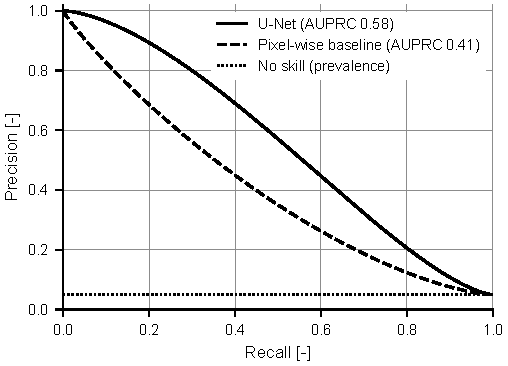
\includegraphics{figures/pr_curves}\hfill
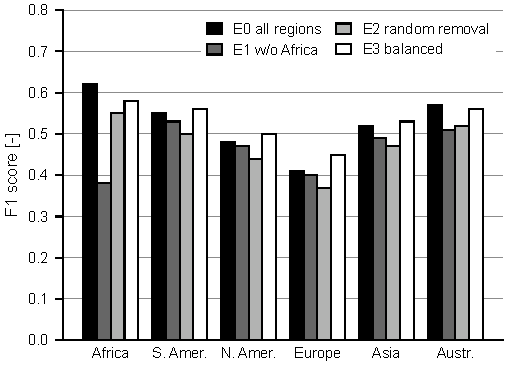
\includegraphics{figures/f1_regions}
\caption{\emph{Left}: precision-recall curves on the test years, all regions (E0); solid = U-Net, dashed = pixel-wise baseline, dotted = no-skill reference. \emph{Right}: F1 per test region for E0 to E3. Illustrative numbers.}
\label{fig:pr}
\end{figure}

\begin{table}[!tb]
\centering\small
\caption{F1 score per test region and experiment (illustrative numbers). Bold: region removed from training.}
\label{tab:res}
\begin{tabular}{lcccccc}
\toprule
Experiment & Africa & S.\ America & N.\ America & Europe & Asia & Australia \\
\midrule
E0 all regions      & 0.62 & 0.55 & 0.48 & 0.41 & 0.52 & 0.57 \\
E1 without Africa   & \textbf{0.38} & 0.53 & 0.47 & 0.40 & 0.49 & 0.51 \\
E2 random removal   & 0.55 & 0.50 & 0.44 & 0.37 & 0.47 & 0.52 \\
E3 balanced         & 0.58 & 0.56 & 0.50 & 0.45 & 0.53 & 0.56 \\
\bottomrule
\end{tabular}
\end{table}

\subsection{Leaving Africa Out (E1)}
\guide{the drop in Africa and its neighbours; Figure~\ref{fig:pr}, right.}
\dummy{21-22}
\dummy{42-43}

\subsection{Random Region Removal (E2)}
\guide{mean and spread over 3 seeds; is Africa a special case?}
\dummy{23}
\dummy{44-45}

\subsection{Balanced Training (E3)}
\guide{gain in the weakest regions and cost in the strongest.}
\dummy{24}
\dummy{46-47}

\begin{figure}[!tb]
\centering\placeholder{\linewidth}{60mm}{Figure to come: predicted vs observed burned area in Africa for one test season, E0 vs E1 (task 3.2).}
\caption{Predicted burn probability and observed burned pixels in Africa, one test season. \emph{Left}: E0; \emph{right}: E1. Own figure.}
\label{fig:maps}
\end{figure}

\subsection{Temporal Shift (Bonus)}
\guide{only if task 5.1 is done: train on early years, test on recent ones.}
\dummy{25}

% =============================================================================
\section{Discussion}
\guide{what the drop says about fire regimes; limits (coarse 0.25\,deg grid, one target product, few seeds); compute time per experiment.}
\dummy{26-28}
\dummy{48-51}
\dummy{53-55}

% =============================================================================
\section{Conclusion}
\guide{the answer to the question in two sentences, then the next step.}
\dummy{29}
\dummy{52}

% =============================================================================
\begin{thebibliography}{9}
\bibitem{seasfire} I.~Karasante \emph{et al.}, ``SeasFire Cube: A global dataset for seasonal fire modeling in the Earth system,'' Zenodo, 2023.
\bibitem{kondylatos} S.~Kondylatos \emph{et al.}, ``Wildfire danger prediction and understanding with deep learning,'' \emph{Geophys.\ Res.\ Lett.}, vol.~49, 2022.
\bibitem{prapas} I.~Prapas \emph{et al.}, ``TeleViT: Teleconnection-driven transformers improve subseasonal to seasonal wildfire forecasting,'' in \emph{Proc.\ ICCV Workshops}, 2023.
\bibitem{wilds} P.~W.~Koh \emph{et al.}, ``WILDS: A benchmark of in-the-wild distribution shifts,'' in \emph{Proc.\ ICML}, 2021.
\bibitem{unet} O.~Ronneberger, P.~Fischer, and T.~Brox, ``U-Net: Convolutional networks for biomedical image segmentation,'' in \emph{Proc.\ MICCAI}, 2015.
\bibitem{focal} T.-Y.~Lin, P.~Goyal, R.~Girshick, K.~He, and P.~Doll\'ar, ``Focal loss for dense object detection,'' in \emph{Proc.\ ICCV}, 2017.
\end{thebibliography}
\end{document}
